%==============================================================================
\section{The problem and the tools used to attack it}\label{sec:prelim}
%==============================================================================

This section defines the SSP, the rule that solves its inner problem, the
grouping view that the whole report is built on, and the two elementary lower
bounds that everything later is measured against. It ends with a self-contained
account of the integer-programming background used in Section~\ref{sec:exact}.

\subsection{The Job Sequencing and Tool Switching Problem}\label{ssec:ssp}

An instance consists of $n$ jobs $J=\rset{1,\dots,n}$, a set of tools $T$, a
magazine capacity $b\in\mathbb{N}$, and for each job $j$ a set of required tools
$T_j\subseteq T$ with $1\le\lvert T_j\rvert\le b$. The requirement
$\lvert T_j\rvert\le b$ is necessary: a job needing more tools than the magazine
holds could never be run. Write $\U=\bigcup_{j\in J}T_j$ for the set of tools that
some job requires. Tools outside $\U$ play no part and are ignored.
If $b>\lvert\U\rvert$, replacing $b$ by $\lvert\U\rvert$ changes no feasible
schedule or insertion cost. We make that preprocessing convention once and henceforth
assume $b\le\lvert\U\rvert$; in particular $q=\lvert\U\rvert-b$ is non-negative.

\begin{definition}[Schedule and switch cost]\label{def:ssp}
A \emph{schedule} is a pair $(\pi,\mathbf{M})$, where $\pi$ is a permutation of $J$
giving the order in which the jobs run, and $\mathbf{M}=(M_1,\dots,M_n)$ gives the
magazine contents at each position. It is feasible when
\[
  \lvert M_i\rvert\le b \quad\text{and}\quad T_{\pi(i)}\subseteq M_i
  \qquad (i=1,\dots,n),
\]
that is, when the magazine never overflows and always holds what the current job
  needs. With $M_0=\varnothing$, its \emph{empty-start cost} is
\[
  \sum_{i=1}^{n}\lvert M_i\setminus M_{i-1}\rvert .
\]
The \emph{free-initial cost} omits the $i=1$ term: the first fill is free and every
later insertion is charged. Throughout the theory $\Zst$ denotes the minimum
free-initial cost; $\Zempty$ denotes the minimum empty-start cost reported by the
computational study.
\end{definition}

Counting insertions rather than removals is the standard cost model. Under a fixed
capacity each insertion into a full magazine forces exactly one removal, so the two
counts differ only at the start of the schedule. Section~\ref{ssec:conv} makes that
difference precise.

The following instance is used as an example throughout the report.

\begin{example}[The $6$-ring]\label{ex:ring}
The \emph{$6$-ring} has six jobs, six tools and capacity $b=3$. Job $j$ requires
$T_j=\rset{j,\,j+1}$, with indices taken modulo $6$, so that $T_6=\rset{6,1}$.
Consecutive jobs share exactly one tool and non-consecutive jobs share none. Its
job--tool incidence matrix, with rows for tools and columns for jobs and a blank
denoting $0$, is
\[
\begin{array}{c|cccccc}
      & 1 & 2 & 3 & 4 & 5 & 6\\\hline
 t_1  & 1 &   &   &   &   & 1\\
 t_2  & 1 & 1 &   &   &   &  \\
 t_3  &   & 1 & 1 &   &   &  \\
 t_4  &   &   & 1 & 1 &   &  \\
 t_5  &   &   &   & 1 & 1 &  \\
 t_6  &   &   &   &   & 1 & 1
\end{array}
\]
Figure~\ref{fig:ring} draws it. Its optima are $\Zempty=6$ empty-start and
$\Zst=3$ free-initial; Section~\ref{ssec:ktns} computes them.
\end{example}

\begin{figure}[h]\centering
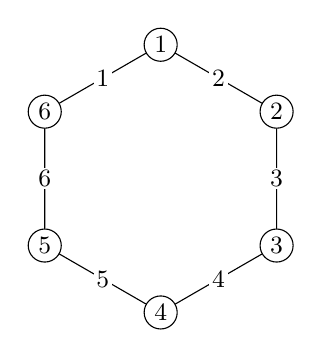
\begin{tikzpicture}[scale=1.7,line cap=round,every node/.style={font=\small}]
  \foreach \i in {1,...,6}{
    \node[draw,circle,fill=white,inner sep=1.6pt] (j\i) at ({90-(\i-1)*60}:1) {$\i$};
  }
  \foreach \a/\b/\t in {1/2/2,2/3/3,3/4/4,4/5/5,5/6/6,6/1/1}{
    \draw (j\a)--(j\b) node[midway,fill=white,inner sep=1pt]{$\t$};
  }
\end{tikzpicture}
\caption{The $6$-ring. The six jobs lie on a cycle. Each edge is labelled by the
single tool its two endpoint jobs share, so job $j$ requires the two tools on the
edges meeting it. Adjacent jobs overlap in one tool; non-adjacent jobs are
tool-disjoint.}\label{fig:ring}
\end{figure}

\subsection{Loading tools for a fixed order}\label{ssec:ktns}

Suppose the order of the jobs is already decided. What remains is to choose the
magazine contents at each position. This inner problem has a closed-form solution.

\begin{proposition}[\citealp{Tang1988}]\label{prop:ktns}
Fix a permutation $\pi$. The following rule produces a magazine sequence of minimum
switch cost. Process the jobs in the order $\pi$. Whenever a required tool is
absent, insert it; if the magazine is full, first remove a tool whose next required
use lies furthest in the future, removing a tool never required again if one
exists. This is the \emph{Keep Tool Needed Soonest} (KTNS) rule. It runs in
$O(n\lvert T\rvert)$ time, and no loading policy for $\pi$ costs less.
\end{proposition}

The proof is in \citet{Tang1988}; \citet{Crama1994} give a second proof through
interval matrices. Write $\KTNS(\pi)$ for its free-initial value (subtracting the
constant first fill from the empty-start count). Since the rule is optimal for every
fixed order,
\[
  \Zst \;=\; \min_{\pi}\ \KTNS(\pi),
\]
so the SSP reduces to a pure sequencing problem. Every method in this report is
some way of searching over orders while delegating the loading to this rule.

\begin{example}[KTNS on the $6$-ring]\label{ex:ktns}
Take the $6$-ring and the cyclic order $1,2,3,4,5,6$. Figure~\ref{fig:ktns} traces
it. The magazine starts empty and holds three tools.

Jobs~1 and~2 need $\rset{1,2}$ and $\rset{2,3}$, so the first magazine is filled
with $\rset{1,2,3}$: three insertions, and this serves both jobs. At position~3,
job~3 needs $\rset{3,4}$. Tool~3 is already loaded, so only tool~4 is inserted, and
one resident tool must leave. This is where the rule does its work. Of the residents
$\rset{1,2,3}$, tool~2 is never required again, while tool~1 is required by job~6 at
the very end. The rule removes tool~2 and keeps tool~1. Positions~4 and~5 repeat the
pattern, inserting one new tool and removing the one whose next use is furthest
away. Position~6 needs $\rset{6,1}$, and both are present, so it is free.

The total is three insertions to fill the magazine plus one at each of positions
$3,4,5$: six insertions, or three once the first fill is not charged. Keeping tool~1
loaded through three positions where it is not used is what the rule buys. A policy
that removed tool~1 at position~3 would have to reload it at position~6 and would
pay seven.
\end{example}

\begin{figure}[t]\centering
\begin{tikzpicture}[x=0.8cm,y=0.8cm,font=\footnotesize]
  \foreach \p/\req in {1/{1{,}2},2/{2{,}3},3/{3{,}4},4/{4{,}5},5/{5{,}6},6/{6{,}1}}{
    \node[font=\footnotesize] at (\p,6.05) {\p};
    \node[font=\scriptsize,text=black!55] at (\p,6.7) {$\{\req\}$};}
  \foreach \t/\y in {1/5,2/4,3/3,4/2,5/1,6/0}{\node[anchor=east,font=\footnotesize] at (0.4,\y) {$t_{\t}$};}
  \foreach \p/\y in {2/5,3/5,4/5,5/5,6/5, 2/4, 2/3,3/3, 4/2, 5/1,6/1, 6/0}{
     \fill[cBlue!20] (\p-0.5,\y-0.5) rectangle (\p+0.5,\y+0.5);}
  \foreach \p/\y in {1/5,1/4,1/3, 3/2, 4/1, 5/0}{
     \fill[cOrange!90] (\p-0.5,\y-0.5) rectangle (\p+0.5,\y+0.5);
     \draw[white,line width=0.9pt] (\p-0.17,\y)--(\p+0.17,\y);
     \draw[white,line width=0.9pt] (\p,\y-0.17)--(\p,\y+0.17);}
  \draw[black!35,step=1] (0.5,-0.5) grid (6.5,5.5);
  \node[font=\scriptsize,text=black!70] at (1,-1.05) {initial fill};
  \node[font=\scriptsize,text=black!70] at (4,-1.05) {three further insertions};
\end{tikzpicture}
\caption{KTNS on the $6$-ring in the order $1,2,3,4,5,6$. Columns are the six
processing positions, with the tools each job needs written above them; rows are the
six tools. A shaded cell means the tool sits in the magazine at that position; a
``$+$'' marks an insertion. Every column holds exactly three tools. Tool~1, in the
top row, is loaded once and kept across all six positions, idle in the middle, so
that it need not be reloaded for job~6. The cost is three insertions to fill the
magazine and three afterwards: six in the empty-start cost, three in the
free-initial cost.}
\label{fig:ktns}
\end{figure}

\begin{remark}[The loading problem is offline caching]\label{rem:belady}
For a fixed order the loading problem is exactly offline paging. The magazine is a
cache of size $b$, position $i$ requests the set $T_{\pi(i)}$, and an insertion is a
cache miss. Proposition~\ref{prop:ktns} is then the tool-switching form of
B\'el\'ady's optimal replacement rule, which removes the item whose next request is
furthest in the future and which minimises misses on any fixed request sequence
\citep{Belady1966}. The comparison is informative. Paging takes the request order as
given; the SSP may reorder the jobs, and it is that freedom which turns a
polynomially solvable caching problem into an NP-hard one.
\end{remark}

\subsection{Configurations}\label{ssec:gtsp}

The magazine, not the job, is the natural unit for what follows.

\begin{definition}[Configuration, cluster, transition cost]\label{def:config}
A \emph{configuration} is a set $C\subseteq\U$ with exactly $\lvert C\rvert=b$
tools. The set of all configurations is written $\confs$. For a job $j$, the
\emph{cluster} $H_j=\rset{C\in\confs : T_j\subseteq C}$ is the set of
configurations able to serve $j$. For two configurations, the \emph{transition
cost} is the number of tools that must be inserted to pass from one to the other,
\[
  d(C,C') \;=\; \lvert C'\setminus C\rvert .
\]
\end{definition}

Restricting attention to full magazines costs nothing. Keeping a tool that might be
useful later never increases the number of insertions, so some optimal schedule
keeps the magazine full at every position whenever $\lvert\U\rvert\ge b$.

Under this view a schedule is a walk $C_{(1)},\dots,C_{(r)}$ through $\confs$ that
visits at least one configuration of every cluster $H_j$, and its cost is
$\sum_l d(C_{(l)},C_{(l+1)})$. That a schedule and such a walk have equal cost is
immediate in one direction: take any schedule, delete repetitions from its sequence
of magazines, and what remains is a walk of the same cost that serves every job. The
converse is Theorem~\ref{thm:grouping} in Section~\ref{ssec:exact}.

The SSP is therefore a generalised travelling-salesman problem over $\confs$, in
which the clusters \emph{overlap}: one configuration can serve many jobs. The
formulation is documented by \citet{Moreira2026}, who attributes it to a 2024 personal
communication by Rafael Colares, Mauricio de Souza and Annegret Wagler. The overlap is what separates it
from the textbook generalised travelling-salesman problem with disjoint clusters
\citep{Noon1993,Fischetti1997,Pop2024}, and it is why the standard reductions for
that problem do not transfer.

\subsection{Grouping the jobs}\label{ssec:jgp}

Section~\ref{ssec:ktns} settled the loading problem, so what remains is the order.
Solving for the order directly is hard, so practice does something indirect. It
first asks a simpler question: which jobs could share a magazine?

\begin{definition}[Feasible group]\label{def:group}
A set of jobs $G\subseteq J$ is a \emph{feasible group} if the tools its jobs need,
taken together, fit in the magazine:
\[
  \Bigl\lvert \bigcup_{j\in G} T_j \Bigr\rvert \;\le\; b .
\]
\end{definition}

A feasible group can be run from start to finish without a single tool change. Load
the tools its jobs need, run them in any order, and only then change anything. This
makes the following question natural.

\begin{definition}[Job Grouping Problem]\label{def:jgp}
The \emph{Job Grouping Problem} (JGP) is the problem of partitioning $J$ into as few
feasible groups as possible. The smallest possible number of groups is written
$\Kst$.
\end{definition}

The JGP ignores order completely. It asks only how the jobs may be divided. It is
itself NP-hard, but it is far easier in practice than the SSP, and it is solved
exactly on every instance size considered here, by the asymmetric-representatives
formulation of \citet{Jans2013} or by the set-covering column generation of
\citet{Crama1994Column}.

Two problems now sit next to each other. The JGP says which jobs may share a
magazine. The SSP asks for an order. The standard heuristic joins them, in three
steps.

\begin{enumerate}[topsep=4pt,itemsep=2pt]
  \item \textbf{Group.} Solve the JGP. This returns $\Kst$ feasible groups
  $G_1,\dots,G_{\Kst}$, and for each group a configuration $C_l$ containing
  everything that group needs.
  \item \textbf{Sequence.} Decide the order of the groups. Moving from
  configuration $C$ to configuration $C'$ costs $d(C,C')$, so finding the cheapest
  order of the $\Kst$ configurations is a travelling-salesman problem on $\Kst$
  points, which is small enough to solve exactly
  \citep{Applegate2006,Helsgaun2015}.
  \item \textbf{Evaluate.} Write out the jobs group by group, in the order chosen in
  step~2, to obtain a single job order. Apply KTNS to that order and report its cost.
\end{enumerate}

This is the method studied throughout this report. It is fast, it is what
practitioners use, and its output is always a feasible schedule, so its cost is never
below $\Zst$.

\begin{example}[The heuristic on the $6$-ring]\label{ex:jgp-ring}
Step~1 returns $\Kst=3$ for the $6$-ring. One optimal grouping is
\[
  G_1=\rset{1,2},\qquad G_2=\rset{3,4},\qquad G_3=\rset{5,6},
\]
whose tool requirements are $\rset{1,2,3}$, $\rset{3,4,5}$ and $\rset{5,6,1}$. Each
has exactly three tools, so each group fixes its configuration with no freedom left:
$C_1=\rset{1,2,3}$, $C_2=\rset{3,4,5}$, $C_3=\rset{5,6,1}$.

Step~2 compares them. Any two share exactly one tool, so moving between any two
costs two insertions. Every order of the three groups costs the same, and step~2 may
return any of them. Take $G_1,G_2,G_3$.

Step~3 writes out the jobs group by group, giving the order $1,2,3,4,5,6$, and
applies KTNS. That is the order traced in Example~\ref{ex:ktns}, and its cost is six
insertions, or three once the first fill is not charged.
\end{example}

Two features of this example matter later.

First, the method does not fully determine its own answer. Step~1 may return several
optimal groupings, step~2 may face ties as it does here, and the order of the jobs
\emph{inside} a group is left open by all three steps. Different choices can give
different costs. Throughout this report the heuristic is read in its most favourable
form: its cost is the best value reachable over all of these choices. This is the
reading that makes a comparison with $\Zst$ meaningful, because any weaker reading
would measure the tie-breaking rule rather than the method.

Second, and less obviously, step~3 does something that step~2 did not anticipate.
That is the subject of the next subsection.

\subsection{Two ways to measure the heuristic}\label{ssec:frames}

Steps~1 and~2 reason entirely in terms of configurations. Each group is assigned one
magazine, and that magazine is imagined to stay loaded while the whole group runs.
Under that picture a schedule is a walk through $\Kst$ configurations, and its cost
is the sum of the transition costs along the walk.

Step~3 does not do this. It discards the configurations, keeps only the job order
they produced, and hands that order to KTNS. KTNS may change the magazine between
any two consecutive jobs, including two jobs of the same group. The group structure
survives only as an ordering of the jobs; it does not constrain the magazine.

The two readings give different numbers. Both appear in the literature without being
distinguished. This report separates them.

\begin{definition}[The walk value and the heuristic value]\label{def:frames}
Let $\mathcal{P}$ range over the partitions of $J$ into $\Kst$ feasible groups. For
each such partition let the configurations be chosen and ordered as cheaply as
possible, and write
\[
  \Hwalk
  \;=\;\min_{\mathcal{P}}\;\min_{\sigma}\;
        \sum_{l=1}^{\Kst-1} d\bigl(C_{\sigma(l)},C_{\sigma(l+1)}\bigr)
\]
for the cheapest such walk. Write $H$ for the cost of the two-phase heuristic as
defined in Section~\ref{ssec:jgp}: the minimum, over the same partitions, over all
orders of the groups and all orders of the jobs within each group, of the KTNS cost
of the resulting job order.
\end{definition}

\begin{remark}[$H$ is an envelope, not the output of an implementation]\label{rem:envelope}
Both $\Hwalk$ and $H$ minimise over every choice the method leaves open: which
minimum-cardinality grouping, which order of the groups, and which order of the jobs
inside each group. They are therefore the \emph{best} value reachable by the two-phase
construction, not the value a particular implementation returns. Any implementation
resolves those choices by some rule and returns a value at least as large, so a bound
proved here for $H$ bounds the best case of the construction and is not by itself an
approximation guarantee for a deterministic implementation of it. The choice is
deliberate --- the alternative measures a tie-breaking rule rather than the method ---
but every gap statement in Section~\ref{sec:gap} should be read with it in mind.
\end{remark}

\begin{proposition}\label{prop:frames}
For every instance, $H\le\Hwalk$.
\end{proposition}

\begin{proof}
Fix a partition and an order of its groups attaining $\Hwalk$. Writing the jobs out
group by group in that order gives a job order. Holding each group's configuration
fixed while its jobs run is one admissible loading for that order, and its cost is
exactly the walk cost. By Proposition~\ref{prop:ktns}, KTNS returns the cheapest
loading for that order, so the KTNS cost is at most the walk cost. Since $H$
minimises over at least this one job order, $H\le\Hwalk$.
\end{proof}

The inequality can be strict, and it is strict on the running example.

\begin{example}[The two values differ on the $6$-ring]\label{ex:frames-ring}
Continue Example~\ref{ex:jgp-ring}. The walk pays three insertions to build
$C_1=\rset{1,2,3}$, then two to reach $C_2=\rset{3,4,5}$, then two to reach
$C_3=\rset{5,6,1}$. That is $\Hwalk=7$, or $4$ free-initial. KTNS on the same job
order costs $6$, or $3$ free-initial. Since $\Zst=3$ free-initial, the heuristic is
\emph{optimal} on the $6$-ring while the walk value is one above the optimum.

Figure~\ref{fig:frames} shows where the two part company. The walk requires the
middle group to run under $C_2=\rset{3,4,5}$ and nothing else. Tool~1 is not in
$C_2$, so it is removed at position~3 and must be reloaded at position~5 for job~6.
KTNS is not bound to $C_2$. It holds $\rset{1,3,4}$ at position~3 and
$\rset{1,4,5}$ at position~4, two different magazines inside one group, each
serving its own job, and so keeps tool~1 loaded throughout. The one re-insertion is
avoided.
\end{example}

\begin{figure}[t]\centering
\begin{tikzpicture}[x=0.8cm,y=0.8cm,font=\footnotesize]
 % ---------------- (a) the configuration walk ----------------
 \begin{scope}
  \node[font=\footnotesize\bfseries,anchor=west] at (0.15,7.6)
     {(a) the walk: one magazine per group};
  \foreach \p/\req in {1/{1{,}2},2/{2{,}3},3/{3{,}4},4/{4{,}5},5/{5{,}6},6/{6{,}1}}{
    \node[font=\footnotesize] at (\p,6.05) {\p};
    \node[font=\scriptsize,text=black!55] at (\p,6.7) {$\{\req\}$};}
  \foreach \t/\y in {1/5,2/4,3/3,4/2,5/1,6/0}{
    \node[anchor=east,font=\footnotesize] at (0.4,\y) {$t_{\t}$};}
  \foreach \p/\y in {1/5,2/5,5/5,6/5, 1/4,2/4, 1/3,2/3,3/3,4/3,
                     3/2,4/2, 3/1,4/1,5/1,6/1, 5/0,6/0}{
     \fill[cBlue!20] (\p-0.5,\y-0.5) rectangle (\p+0.5,\y+0.5);}
  \foreach \p/\y in {1/5,1/4,1/3, 3/2,3/1, 5/5,5/0}{
     \fill[cOrange!90] (\p-0.5,\y-0.5) rectangle (\p+0.5,\y+0.5);
     \draw[white,line width=0.9pt] (\p-0.17,\y)--(\p+0.17,\y);
     \draw[white,line width=0.9pt] (\p,\y-0.17)--(\p,\y+0.17);}
  \draw[black!35,step=1] (0.5,-0.5) grid (6.5,5.5);
  \draw[black!55,semithick,dashed] (2.5,-0.5) -- (2.5,5.5);
  \draw[black!55,semithick,dashed] (4.5,-0.5) -- (4.5,5.5);
  \foreach \x/\g in {1.5/1,3.5/2,5.5/3}{
    \node[font=\scriptsize,text=black!55] at (\x,-1.05) {$G_{\g}$};}
  \node[font=\scriptsize,text=black!70,anchor=west] at (0.5,-1.8)
     {seven insertions};
 \end{scope}
 % ---------------- (b) KTNS on the same job order ----------------
 \begin{scope}[xshift=7.7cm]
  \node[font=\footnotesize\bfseries,anchor=west] at (0.15,7.6)
     {(b) KTNS on the same job order};
  \foreach \p/\req in {1/{1{,}2},2/{2{,}3},3/{3{,}4},4/{4{,}5},5/{5{,}6},6/{6{,}1}}{
    \node[font=\footnotesize] at (\p,6.05) {\p};
    \node[font=\scriptsize,text=black!55] at (\p,6.7) {$\{\req\}$};}
  \foreach \t/\y in {1/5,2/4,3/3,4/2,5/1,6/0}{
    \node[anchor=east,font=\footnotesize] at (0.4,\y) {$t_{\t}$};}
  \foreach \p/\y in {1/5,2/5,3/5,4/5,5/5,6/5, 1/4,2/4, 1/3,2/3,3/3,
                     3/2,4/2, 4/1,5/1,6/1, 5/0,6/0}{
     \fill[cBlue!20] (\p-0.5,\y-0.5) rectangle (\p+0.5,\y+0.5);}
  \foreach \p/\y in {1/5,1/4,1/3, 3/2, 4/1, 5/0}{
     \fill[cOrange!90] (\p-0.5,\y-0.5) rectangle (\p+0.5,\y+0.5);
     \draw[white,line width=0.9pt] (\p-0.17,\y)--(\p+0.17,\y);
     \draw[white,line width=0.9pt] (\p,\y-0.17)--(\p,\y+0.17);}
  \draw[black!35,step=1] (0.5,-0.5) grid (6.5,5.5);
  \draw[black!55,semithick,dashed] (2.5,-0.5) -- (2.5,5.5);
  \draw[black!55,semithick,dashed] (4.5,-0.5) -- (4.5,5.5);
  \foreach \x/\g in {1.5/1,3.5/2,5.5/3}{
    \node[font=\scriptsize,text=black!55] at (\x,-1.05) {$G_{\g}$};}
  \node[font=\scriptsize,text=black!70,anchor=west] at (0.5,-1.8)
     {six insertions};
 \end{scope}
\end{tikzpicture}
\caption{The same grouping of the $6$-ring, measured two ways. Columns are the six
processing positions, with the tools each job needs above them; rows are the six
tools. A shaded cell means the tool sits in the magazine at that position; a
``$+$'' marks an insertion. The dashed lines separate the three groups. In (a) each
group runs under one fixed magazine, so tool~1, in the top row, is removed at
position~3 and reloaded at position~5 for job~6: seven insertions. In (b) KTNS may
change the magazine inside a group, so tool~1 is loaded once and kept across all six
positions, and the count is six. That single re-insertion is the whole difference
between $\Hwalk$ and $H$.}
\label{fig:frames}
\end{figure}

\begin{remark}[Why the distinction is kept throughout]\label{rem:frames}
It would be simpler to work with $\Hwalk$ alone. It has a clean description, a
shortest walk through $\Kst$ configurations, and the structural results of
Section~\ref{sec:gap} are naturally proved about it.

That simplification is not available, for two reasons. The first is that $\Hwalk$ is
not what the method returns. A practitioner running the three steps of
Section~\ref{ssec:jgp} obtains $H$, so any statement about how far the method can be
from optimal must be a statement about $H$. The second is that the two differ on
exactly the instances most often used as examples, as Example~\ref{ex:frames-ring}
shows.

Every result in Section~\ref{sec:gap} therefore names the value it is about.
Proposition~\ref{prop:frames} carries upper bounds in one direction: anything proved
to bound $\Hwalk$ from above also bounds $H$. Nothing transfers in the other
direction. In particular, an instance on which $\Hwalk$ exceeds $\Zst$ is not by
itself an instance on which the heuristic is suboptimal.
\end{remark}

\subsection{Two lower bounds}\label{ssec:lb}

Two elementary bounds on $\Zst$ recur throughout. Both are stated in the
free-initial cost of Section~\ref{ssec:conv}, which does not charge the first
magazine fill. Write $q=\lvert\U\rvert-b$ for the number of used tools in excess of
the capacity; the quantity appears often enough to deserve a name.

\begin{proposition}[Grouping bound]\label{prop:lb1}
$\Zst\ge\Kst-1$.
\end{proposition}

\begin{proof}
Fix any schedule and list its magazine states. Collapse each run of equal
consecutive states to a single representative, giving a sequence
$C_{(1)},\dots,C_{(r)}$ in which consecutive entries differ. Every job is served by
some state, hence by some $C_{(l)}$. Assign each job to one configuration containing
its requirement. This partitions $J$ into at most $r$ groups, each with combined
requirement inside one configuration and therefore of size at most $b$. That is a
feasible grouping, so $r\ge\Kst$. Each of the $r-1$ transitions inserts at least one
tool, so the free-initial cost is at least $r-1\ge\Kst-1$.
\end{proof}

\begin{proposition}[Coverage bound]\label{prop:lb2}
$\Zst\ge\lvert\U\rvert-b=q$.
\end{proposition}

\begin{proof}
Every tool of $\U$ is required by some job, so it occupies the magazine at some
position, so it is inserted at least once unless it belongs to the first fill. The
first fill holds at most $b$ tools. Hence at least $\lvert\U\rvert-b$ insertions are
made beyond the first fill.
\end{proof}

\begin{corollary}\label{cor:lb}
$\Zst\ge\max\rset{\Kst-1,\ q}$.
\end{corollary}

Neither bound dominates the other, and their maximum is not always attained. On the
$6$-ring, $\Kst-1=2$ while $q=6-3=3$, so the coverage bound is tight and the
grouping bound is slack. On instances built from many nearly tool-disjoint groups
the reverse holds. And both can be slack at once: the eight-job instance with
$T_j=\rset{j,j+1,j+2}$ modulo $8$ and $b=4$ has $\Kst-1=3$ and $q=4$, but
$\Zst=5$.\footnote{Verified by exhaustive computation; see
Appendix~\ref{app:verify}.}

The coverage bound $q$ deserves particular attention, because
Section~\ref{ssec:compact} shows that the SSPMF model---the strongest of the three
compact baselines reimplemented here---has a linear relaxation exactly equal to it
when every declared tool is used. It is therefore both an elementary counting
argument and the limit of the campaign's compact baseline set; more recent compact
models such as JGSMF \citep{Akhundov2024} are outside that comparison.

\subsection{Cost conventions}\label{ssec:conv}

\begin{definition}[Empty-start and free-initial costs]\label{def:conv}
The \emph{empty-start} cost counts every insertion, starting from an empty magazine
as in Definition~\ref{def:ssp}. The \emph{free-initial} cost does not charge the
first fill.
\end{definition}

\begin{proposition}[Convention identity]\label{prop:conv}
For every schedule,
\[
  \text{cost}_{\mathrm{empty}}
  \;=\;\text{cost}_{\mathrm{free}}+\lvert M_1\rvert.
\]
Moreover, an optimum may be chosen with a full first magazine, and therefore
$\Zempty=\Zst+b$ under the standing preprocessing convention (equivalently, the
shift is $\min(b,\lvert\U\rvert)$ in the original input notation).
\end{proposition}

\begin{proof}
The two sums differ only by their $i=1$ term, which is
$\lvert M_1\setminus M_0\rvert=\lvert M_1\rvert$. For any fixed order, unused slots
can be filled at the first position with tools chosen by the KTNS next-use rule;
retaining such a tool cannot create an insertion, so some optimum has
$\lvert M_1\rvert=b$. Minimising the identity over full-first optimal loadings gives
the relation between the two optima.
\end{proof}

The shift is a constant for a given instance. Three consequences are used later.
Differences such as $H-\Zst$ are the same in both conventions. Ratios such as
$H/\Zst$ are not, so a ratio is meaningless unless the convention is named. And when
objective values produced by different formulations are compared, they must first be
brought to a common convention; Section~\ref{ssec:validation} describes how the
computational study does this.

\subsection{Background on integer programming}\label{ssec:toolkit}

Section~\ref{sec:exact} builds two exact methods, and both rest on a small body of
standard material. It is set out here, with the examples drawn from the
SSP rather than from generic instances. A reader familiar with integer programming
may go directly to Section~\ref{sec:sota}.

\paragraph{Integer linear programs.}
An \emph{integer linear program} minimises a linear function of decision variables
subject to linear constraints, with some variables required to take whole-number
values. In this report those are almost always $0/1$ variables encoding a discrete
choice: $x_{ij}=1$ when job $j$ runs immediately after job $i$, or $g_{t,i}=1$ when
tool $t$ occupies the magazine at position $i$.

A small example makes the shape concrete. Suppose the order of the jobs is already
fixed and only the loading is to be decided. Let $g_{t,i}\in\rset{0,1}$ say whether
tool $t$ is in the magazine at position $i$, and let $s_{t,i}\ge0$ count an insertion
of $t$ at position $i$. The loading problem is then
\[
\begin{aligned}
  \min\quad & \sum_{t,i}s_{t,i}\\
  \text{subject to}\quad
  & g_{t,i}=1 && \text{for every } t\in T_{\pi(i)},\\
  & \textstyle\sum_{t}g_{t,i}\le b && \text{for every position } i,\\
  & s_{t,i}\ge g_{t,i}-g_{t,i-1},\quad s_{t,i}\ge0 && \text{for every } t,i,
\end{aligned}
\]
with $g_{t,0}=0$. The first family forces the current job's tools to be present, the
second is the capacity limit, and the third charges an insertion whenever a tool is
in the magazine at position $i$ but was not at position $i-1$. This model returns to
the report as the Benders subproblem in Section~\ref{ssec:bbc}.

\paragraph{The linear relaxation and the integrality gap.}
Dropping the integrality requirement leaves the \emph{linear relaxation}, an
ordinary linear program. Linear programs are solved efficiently, and because the
relaxation permits everything the integer program permits and more, its optimum is a
\emph{lower bound} on the integer optimum. The difference between the two is the
\emph{integrality gap}. A formulation whose gap is small is called \emph{strong}.

Strength is not automatic, and the SSP gives the extreme illustration.
\citet{Laporte2004} showed that the linear relaxation of the original formulation of
\citet{Tang1988} has optimum $0$ on every instance, whatever the true optimum: the
fractional solution that spreads every job evenly across every position satisfies all
the constraints at zero cost. A bound of $0$ is useless, and much of the
exact-methods literature reviewed in Section~\ref{sec:sota} is an attempt to repair
this.

\paragraph{Branch and bound.}
A bound becomes a proof of optimality through search. Branch and bound solves the
relaxation; if the answer is integral it is optimal and the search stops. Otherwise
some variable takes a fractional value, and the problem is split into two
subproblems, one forcing that variable up and one forcing it down. Every integer
solution survives in one of the two, so nothing is lost. The subproblems are
explored recursively, and a subproblem is discarded as soon as its relaxation bound
is no better than the best complete solution already found.

Two quantities therefore govern how long the search takes. The \emph{incumbent} is
the best complete solution found so far, and it gives an upper bound. The
\emph{dual bound} is the best lower bound over the unexplored subproblems. The
search ends when they meet. It matters which of the two is lagging, and
Section~\ref{sec:disc} returns to this, because for the SSP it is almost always the
dual bound.

\paragraph{Cutting planes.}
A \emph{cut} is a linear inequality satisfied by every integer solution but violated
by the current fractional one. Adding it removes that fractional point without
removing any genuine solution, so the relaxation becomes stronger. Doing this
repeatedly before branching, and again at the nodes of the tree, is
\emph{branch and cut}. It is what commercial solvers such as CPLEX do internally, and
it is the framework into which the Benders algorithm of Section~\ref{ssec:bbc} is
embedded.

A cut may be added as a \emph{lazy constraint}, checked only when a candidate
integer solution appears, or as a \emph{user cut}, added at fractional points during
the search. The distinction matters for the SSP and is measured in
Section~\ref{ssec:results-bbc}.

\paragraph{Duality, and what dual prices mean.}
Every linear program has a partner, its \emph{dual}, with the same optimal value.
The dual has one variable per constraint of the original, and at an optimal solution
that variable is the \emph{price} of the constraint: the rate at which the optimum
would change if the constraint were relaxed slightly.

In the loading program above, the dual variable attached to ``tool $t$ must be
present at position $i$'' measures how much that requirement costs. This is not an
abstraction; it is precisely what the Benders algorithm reads off in order to build
its cuts, and it is available at no extra cost from the same solve. Duality also
supplies a certificate: any feasible solution of the dual gives a valid lower bound
on the original problem, whether or not it is optimal.

\paragraph{Total unimodularity.}
Some integer programs have no integrality gap at all. If the constraint matrix is
\emph{totally unimodular}, meaning every square submatrix has determinant $0$, $1$ or
$-1$, then the vertices of the relaxation are integral, and solving the linear
program already solves the integer program. The loading program above has this
property: its matrix has the consecutive-ones structure, which is totally unimodular.
That is a second proof that the loading problem is easy, and it is the reason the
Benders subproblem in Section~\ref{ssec:bbc} can be solved as a linear program with
no loss.

\paragraph{Benders decomposition.}
Some problems split into a hard part and a part that becomes easy once the hard part
is fixed. The SSP is one: choose the order, which is hard, and then load the tools,
which is easy. Benders decomposition exploits this.

The \emph{master problem} contains only the hard variables, with the cost of the easy
part replaced by a single variable $\theta$ that starts optimistically low. Given a
candidate solution of the master, the easy \emph{subproblem} is solved exactly. If
its true cost exceeds $\theta$, then $\theta$ was lying, and one linear inequality is
added to the master to say so. The inequality is constructed from the subproblem's
dual solution, and it is valid for every master solution, not only the current one.
Each such cut removes the current over-optimistic guess without removing any genuine
schedule. Repeating drives $\theta$ upward until it equals the true cost, at which
point the master solution is optimal. Figure~\ref{fig:benders} in
Section~\ref{ssec:bbc} draws the loop.

Two variants are relevant. In \emph{logic-based} Benders decomposition
\citep{Hooker2003} the subproblem is settled by a combinatorial algorithm rather than
by linear-programming duality, and the cut is derived from the algorithm's answer. In
\emph{combinatorial} Benders decomposition \citep{Codato2006} the cuts are
combinatorial statements about which choices can occur together. Both appear in
Section~\ref{ssec:bbc}, because KTNS is exactly such a combinatorial oracle.

\paragraph{Column generation and branch-and-price.}
Column generation runs the same idea in reverse. Some formulations have very few
constraints but astronomically many variables, one per configuration, say. Such a
model cannot be written out. Instead a \emph{restricted master problem} is kept over
a small pool of variables and solved. A separate \emph{pricing problem} then asks
whether any variable currently omitted would improve the solution if it were added.
The pricing problem searches the full variable space using the current dual prices,
and returns the most promising variable, called a \emph{column}. The restricted
master is re-solved with it included, and the loop repeats. When the pricing problem
reports that no improving column exists, the restricted master has the same optimal
value as the full model.

Wrapping this inside branch and bound gives \emph{branch-and-price}
\citep{Barnhart1998,Lubbecke2005}. There is one difficulty. Branching on a single
column is usually ineffective and forces the pricing problem to carry a growing list
of forbidden columns, which changes its structure. A branching rule that leaves the
pricing problem structurally unchanged is called \emph{robust}, and
Section~\ref{ssec:pos} uses one.
